
\section{Tools}
\index{secrets!tools}

This interface was designed to allow the expansion of resources.
The visibility of the window \texttt{Tools} can be changed using \texttt{CTRL + F8}.
This interface contains many useful features that will make your life easier.

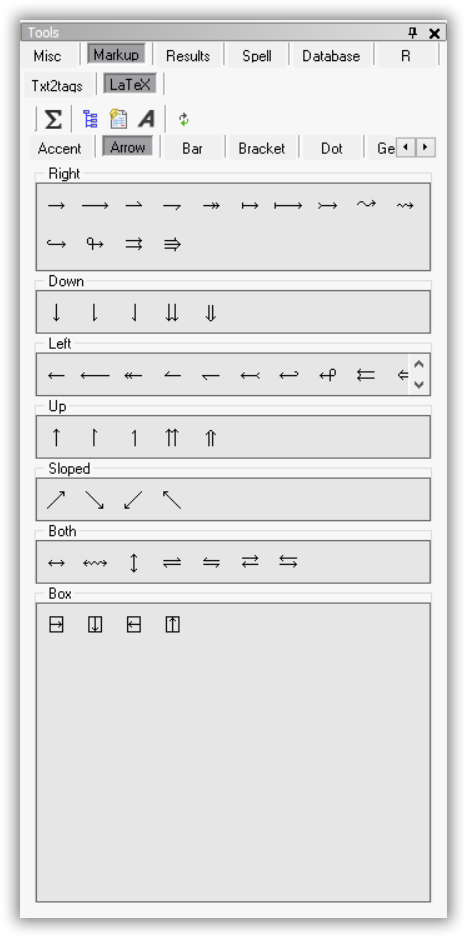
\includegraphics[scale=0.50]{./res/tools_markup_latex_arrows.png}
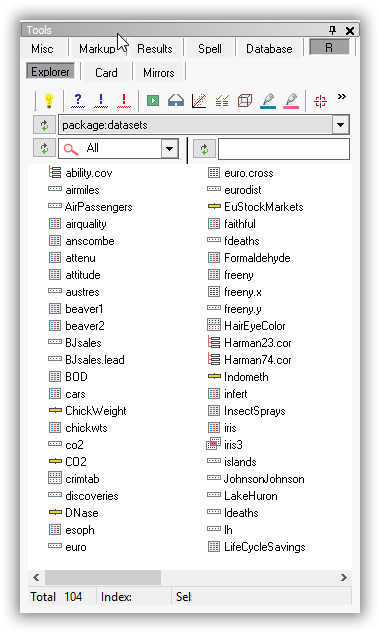
\includegraphics[scale=0.50]{./res/tools_r_explorer.png}
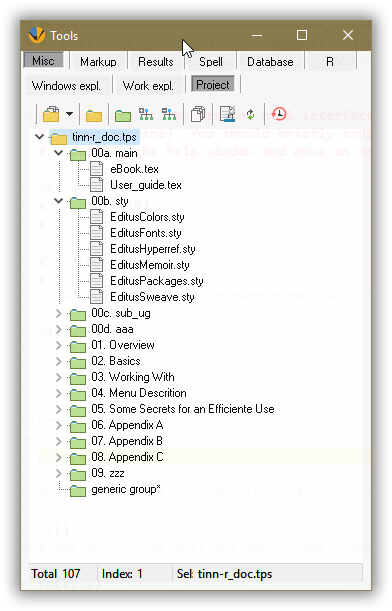
\includegraphics[scale=0.50]{./res/tools_misc_project.png}

\subsection{Project}
\index{secrets!project}

Project allows you to organize different types of files in a hierarchical manner.

Even though your project can be found on the main menu bar, it is easier to work with it using the tools window.
Press \texttt{CTRL + F8} and the tools window will open. Click \texttt{Misc/Project}.

Beginning from the left, the first icon opens up a window where you can search for project files you want to work on.
This file has an extension \texttt{.tps}. Otherwise, go to the next icon to open a new project.

When you click on that project a window will open, allowing you to choose the folder where the project will be stored.

The tree is composed by groups connected at the node level. Groups will contain files with something in common.
For example, if you are writing a package, one group might contain all data files,
another the demo files, another the \RR{} files, and so on. The third box contains three icons.
The first allows you to create new groups and also rename the  deleted groups.
The fourth box (sixth icon) allows you to  open a project or its parts.

The next icon allows you to open a text file with the path corresponding to all files in the project.
This functionality is useful when you move the whole project to another computer.
The path on the other computer may be different from your computer, and so you have to change the corresponding paths.
Save it and start working on the same project on that computer.
You may use the search and replace options to perform that change in paths.

%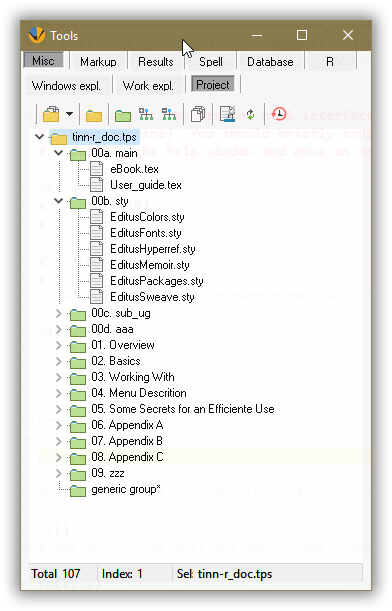
\includegraphics[scale=0.50]{./res/tools_misc_project.png}

\subsection{Database}
\index{secrets!database}

\paragraph{}\textbf{Shortcuts}\\
\index{secrets!database!shortcuts}

You then go to \texttt{Tools/Database} as you click on the box, a small window will open with five tabs.
The first is \texttt{Shortcuts}. There is a long list of commands, some with a shortcut already configured
as a default while other shortcuts can be configured by the user as needed.
You may configure the shortcuts that you are used to. However,
if they are already in use by the Windows operating system, they won't work.
The use of shortcuts can improve the efficiency of your work. You can also have more than one shortcut table.

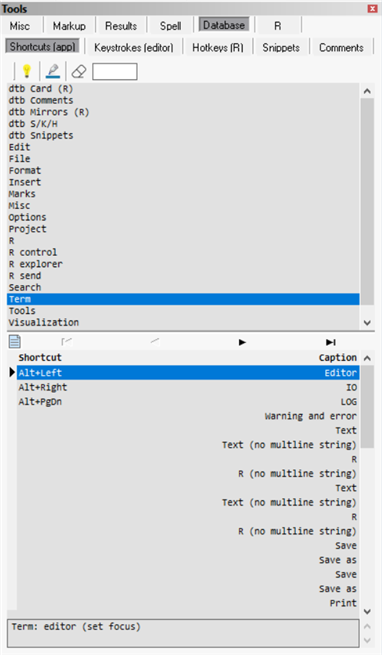
\includegraphics[scale=0.50]{./res/tools_database_shortcuts.png}~~
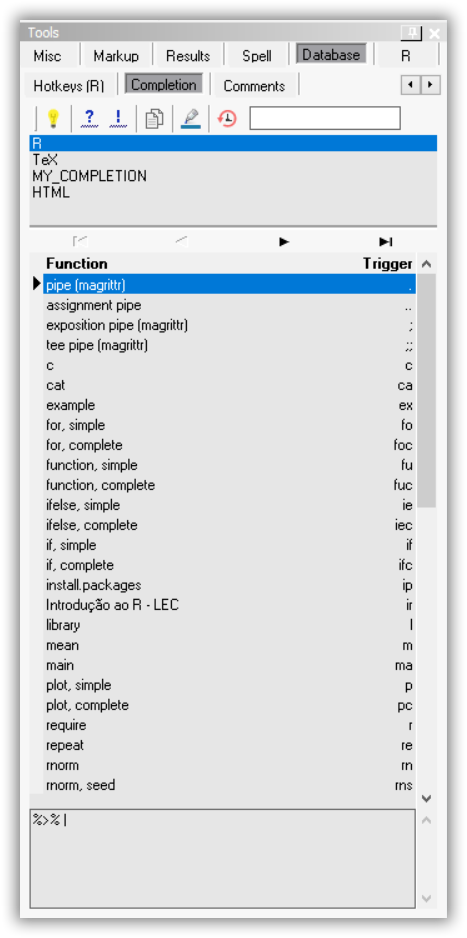
\includegraphics[scale=0.50]{./res/tools_database_completion.png}~~
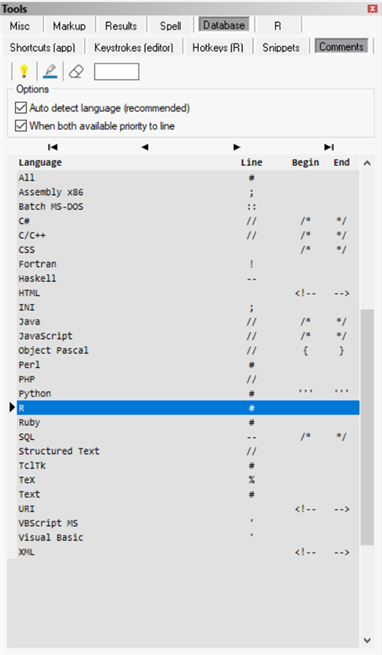
\includegraphics[scale=0.50]{./res/tools_database_comments.png} \\

\paragraph{}\textbf{Completion}\\
\index{secrets!database!completion}

Completion will help you speed up the process of writing \textbf{anything from any language}.
It allows you to personalize its database so that every function, script or text that you
frequently use can be automatically inserted in your script through the click of a button or trigger.

%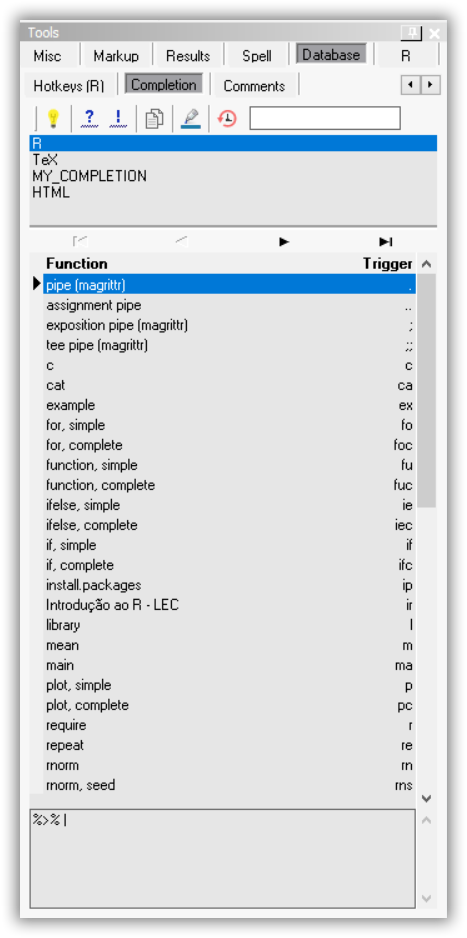
\includegraphics[scale=0.50]{./res/tools_database_completion.png}

Let us start by using completion with the functions which are already in the default database.
First, click on \texttt{Tools/Database/Completion}. A window will open showing all the functions saved in the
database at the bottom of the window. Now click on the fourth icon \texttt{Completion: edit}.
Another window will open, the group to which the function belongs being marked under \texttt{Group},
the function being marked under \texttt{Function} and the trigger under \texttt{Trigger}.

Now open a new file (\texttt{CTRL + N}) and write \texttt{rn} which is the \texttt{trigger for the function rnorm}
and then press \texttt{CTRL + J} or click on \texttt{Insert/Completion} at the main menu.

Now, suppose that you have a section of a script which you use very often when writing scripts.
For example, imagine the following script: x $<$- rnorm(50); y $<$- rnorm(50) which generates
two pseudo-random normal vectors for x- and y-coordinates.

You then select and copy it to the clipboard, click again on the main menu at
\texttt{Tools/Database/Completion} and at the bottom of window click \texttt{New}.
Now, at the top in \texttt{Group} type the name of the group, in this case let the name be \texttt{Examples},
it means that every other example could be saved under this group. In \texttt{Function} type the name of this
specific function, for example, \texttt{norm}, and then type the trigger of this function you are just creating,
say, \texttt{nm} and in complete paste what you copied. Finally click on \texttt{Save} at the bottom of the window.
Now go to your text type nm and press \texttt{CTRL + J},
that part of the script will appear on your text. Did you get the idea?

\paragraph{}\textbf{Comments}\\
The \textit{Comments} resource is very simple and allows high level
of user customization.

From version 3.0.1.0 Tinn-R automatically recognizes the
language of the file on focus. Further, inside the file
- if it is a syntax a multi-highlighter (complex syntax) - which language of
the line where the cursor (or selection) is found.

This identification is done automatically if (and only if) the option
\textit{(x) Auto detect language (recomended)} is checked. Otherwise
the user is forcing the application to use the comments of the selected language
(indicator arrow).

Selected code snippets involving more than one language will not be commented/uncommented
and a warning message is issued. That is, you must select only the snippet of a single language.

\newpage
\subsection{R}
\index{secrets!R}

\paragraph{}\textbf{Explorer}\\
\index{secrets!R!explorer}

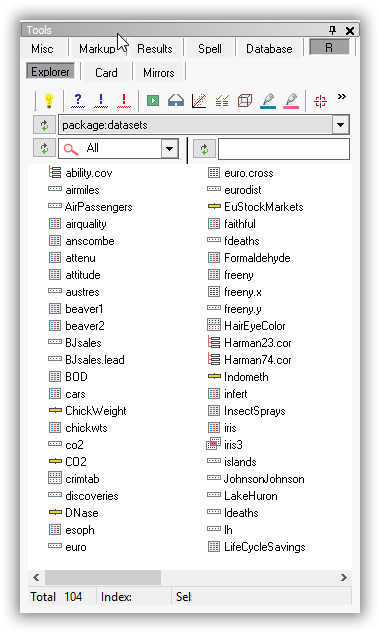
\includegraphics[scale=0.50]{./res/tools_r_explorer.png} \\

This interface has its own pop-up menu, toolbar and three combo box.
The pop-up menu and toolbar contain the most common actions related to an object explorer.

The button \textit{R explorer: refresh environment} sends an instruction to
\RR{} environment requesting the list of all loaded packages in the current
session. The result is shown inside a graphical classified list. When one
of these is selected, the graphical list (and structure) of the objects
are shown.

There are two options of filter: type of objects and any sequence of
characters associated with the names of the objects.

It is possible to remove visible objects of the user workspace (.GlobalEnv)
using the key \textit{Delete}. To do this, select an object and type
\textit{Delete}.

A double click in any selected object will add its name to the editor.
If the object is dragged to the editor interface, the textual description
of the object is always shown in a new file. It is useful to know the
sources of functions and to see data objects (vectors, frames, list, etc).

\newpage
\paragraph{}\textbf{Card}\\
\index{secrets!card (R)}

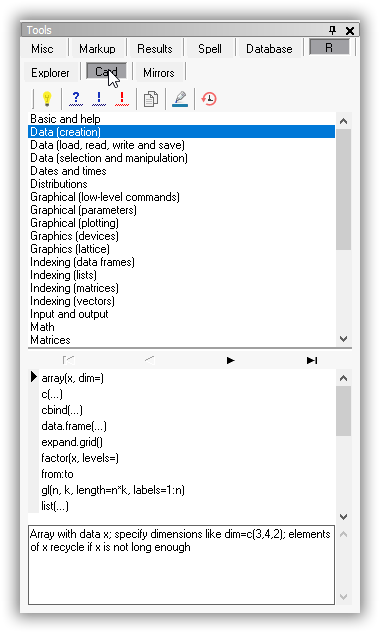
\includegraphics[scale=0.50]{./res/tools_r_card.png} \\

The \textit{card} is a database of distributions, mathematical functions, graphical and statistical functions used in \RR{}.
The main goal of this card is to serve as a means of consultation for the most frequently used commands.
A double mouse click will insert your selection in the text you are editing.

\newpage
\paragraph{}\textbf{Mirrors}\\
\index{R!mirror}
\index{R!set mirror}
\index{R!mirrors}

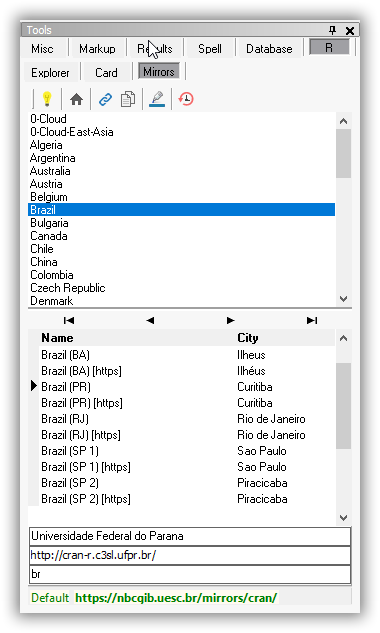
\includegraphics[scale=0.50]{./res/tools_r_mirrors.png} \\

The \textit{mirrors} is an interface that allows the user to manage the repositories (or mirrors) of \RR{}.
You should always choose a repository physically closest to where you are,
so that, the Web communication tends to be faster and more efficient.

The default mirror is the University \href{http://cran.at.r-project.org/}{Wien}
(Austria).
Consider that this is the central mirror of CRAN.

The reasons for the Tinn-R always set a repository (assets) are two:
\begin{itemize}
   \item To prevent \RR{} keeps asking which repository you want to use in each session;
   \item Workaround of intermittency (only related to \texttt{Rterm}) not always showing the dialog for selecting the repository.
    That is, sometimes the dialog is displayed and not others. The cause of this intermittency is still unknown.
\end{itemize}

One important thing to be done is to set a \RR{} mirror as close as possible to where you work.
For that, first click on \texttt{CTRL + F8}.
This opens the \texttt{Tools} window, then click on \texttt{R/Mirrors}.
Select the \RR{} mirror and push the button that shows an hourglass in the taskbar.
The chosen repository will be the new default for all actions dependent repository
(install packages, upgrade packages, etc).

R repositories are little changed with the passage of time.
Thus, the database \texttt{Rmirros.xml} not need to be updated frequently.
However, there are options that make the update whenever the user deems necessary:
\begin{itemize}
   \item Button whose icon is a house on the taskbar Tools/R/Mirrors;
   \item Menu R/Update mirrors.
\end{itemize}
